%%%%%%%%%%%%%%%%%%%%%%%%%%%%%%%%%%%%
% KTHEEtitlepage_ex.tex
%
% Example of how to use the KTHEEtitlepage package.
% 
% Mats Bengtsson,  7/8 2006
%%%%%%%%%%%%%%%%%%%%%%%%%%%%%%%%%%%%
\documentclass[12pt,a4paper]{article}

\usepackage{filecontents,lipsum}
\usepackage[noadjust]{cite}
\usepackage{graphicx}
\usepackage[nonumberlist,acronym,shortcuts]{glossaries}
\graphicspath{{Images/}}

\usepackage[exjobb]{KTHEEtitlepage}
%\renewcommand{\cftsecleader}{\cftdotfill{\cftdotsep}}

% Packages used in the main document for this particular example:
\usepackage{url}
\usepackage{tocloft}
\renewcommand\listfigurename{List of Figures}
\renewcommand\listtablename{List of Tables}



\usepackage{hyperref}
%\usepackage{acro}
\hypersetup{%
	pdfborder = {0 0 0}
}
\usepackage[exjobb]{KTHEEtitlepage}

 \newacronym{asip}{ASIP}{Application Specific Instruction-set Processors}
 \newacronym{ebnf}{EBNF}{Extended Backus Naur Form}
 \newacronym{cpri}{CPRI}{Common Public Radio Interface}
 \newacronym{osi}{OSI}{Open Systems Interconnect model}
 \newacronym{gpp}{GPP}{General Purpose Processor}
 \newacronym{asic}{ASIC}{Application Specific Integrated Circuit}
 \newacronym{tlm}{TLM}{Transaction Level Modeling}
 \newacronym{pla}{PLA}{Programmable Logic Array}
 \newacronym{fpga}{FPGA}{Field Programmable Gate Arrays}
 \newacronym{rbs}{RBS}{Radio Base Station}
 \newacronym{ieee}{IEEE}{Institute of Electrical and Electronics Engineers}
 
 
 
 
 
 

\makeglossaries

\begin{document}
% Information to appear on the title page:
\ititle{Reconfigurable hardware programming in a protocol processor unit}
\isubtitle{}
\iauthor{- Sunil Kallur Ramegowda}
\idate{2015}
\irefnr{IR-EE-Dummy 2000:099}

\iaddress{ICT Labs\\
	Major in Embedded Platforms\\
		Kungliga Tekniska H�gskolan}
		\makeititle

		% Everything below is exactly as for a normal document and 
		% the layout of that document should not be affected in any
		% way by the title page.

		\title{Reconfigurable hardware programming in a protocol processor unit}
		\author{Sunil Kallur Ramegowda}

		\maketitle
		\pagenumbering{roman}
       
  		\begin{abstract}
		
        Reconfigurable hardware architectures are the topic of research for many years.Programming such architectures requires the design of custom compilers to generate the required files for the architecture.
        
        A protocol processor,in general processes the packets according to the protocol.There are number of protocols like Ethernet,\acs{cpri} to define how the data has to be sent and received between the source and destination points. Data packets can be processed using the generic processors programmed in software,but hardware processing is always energy efficient.\\  
        
        A compiler/mapper is developed in this thesis work. The language application was developed using a parser generator tool called Antlr.The grammar was written in \acs{ebnf} and the corresponding language was used to describe the architecture and the protocols. The tool will generate the hardware model and their interconnection in SystemC based on the protocol description.\\ 
        
        The complete system was verified by integrating the Ethernet protocol.Parts of the protocol implementation in SystemC was also considered in the work.The system is verified for different protocols.The framework works based on the user defined description of the protocol. \\
        
        Future work involves the integration of further protocols into the system and then adapt the language to further involve all the future requirements.The concept of mapping can be used to design the hardware blocks and their interconnections in different languages. 
        
        
		\end{abstract}
        \phantomsection
		\addcontentsline{toc}{section}{Abstract}
       	\cleardoublepage

        %\renewcommand\contentsname{\centerline{\underline{\underline{Table of Contents}}}}
		\phantomsection
        \tableofcontents
		%\addcontentsline{toc}{section}{Table of contents}
		\cleardoublepage
        
        % abbreviations
        \phantomsection
        \addcontentsline{toc}{section}{Abbreviations}
        \printglossary[type=\acronymtype,title=Abbreviations]
        \cleardoublepage

		\phantomsection
		\listoffigures
		\addcontentsline{toc}{section}{List of Figures}
		\cleardoublepage

		\phantomsection
        \listoftables
		\addcontentsline{toc}{section}{List of Tables}
		\clearpage

		\pagenumbering{arabic}
         
       \section{Introduction}

		A set of digital rules define the communication strategy between digital systems.There are many rules which makes the communication possible between systems.Over the decades the rules have evolved into standards.The rules are called as Protocols in communication systems.The \gls{osi} partition the communication system into 7 abstraction layers.There are different protocols for each layers of abstraction. The software and/or hardware changes based on the protocol chosen to process the message and extract the relevant information at each layer of abstraction. The hardware solutions based on a \gls{gpp}  or an \gls{asic} exists \cite{5335678}\cite{558379}.GPP will have more flexibility but are less energy efficient when compared to \acs{asic} which are less flexible and most energy efficient. \acs{asip} or domain specific processors are more suitable for the protocol processing task and depending on their architectural characteristics they allow varying degrees of trade-off between flexibility and energy-efficiency\cite{1106752}.Resource and performance varies depending on the reconfigurable architecture and its level of abstraction\cite{6868627}.\\   

		The design of reconfigurable hardware architecture requires the compiler to produce the configuration or the hardware compatible code.These files can be produced on run time when the application is running or in a static way before the application is made to run. The complexity of the system depends on the selected design.The hardware for processing the different protocols can be made reconfigurable.Investigation and design of such a concept is performed in this thesis work.\\ 

		The reconfigurable hardware is modeled in SystemC language using \acs{tlm}. The configuration files required for the reconfiguration is obtained by parsing the description of protocols using the language defined by the Grammar.The Antlr tool is used for building the base parser file for the defined grammar and then the required functions are written to output the complete system and configuration files. 
        

		\clearpage
		\subsection{Background}
		In 1960 Gerald Estrin, proposed the idea of a fixed plus variable structure computer \cite{1114865}.It consisted of a fixed processor and an array of reconfigurable hardware which was controlled by the fixed processor.Even though the idea was demonstrated with a proof,the industry did not consider to further innovate in these field and till 1980's there were no significant developments. In  1985,the reconfigurable \gls{pla} was patented\cite{page1985re}.Innovation in \acs{pla}'s further continued with the commercially available \gls{fpga} in today's market.\\

		Ericsson AB is a market leader in the radio base station equipments.There are different protocols being used for communication in the Radio Base Station (RBS) units.Ethernet standard explained by \acs{ieee} in 802.3 standard defines the protocol for 10Gbit transfer which is mainly used for communication between the silicon chips. Other protocols include \gls{cpri},Serial Rapid IO(SRIO),Xio(Ericsson Specific protocol) for reliable communication between chips at high data rate.Most of these protocols in MAC layer of abstraction have common hardware units. Ericsson design and manufacture Custom \acs{asic} chips for these protocols.The common functions which can be used by different protocols for designing a reconfigurable hardware architecture which will minimize the cost and will provide more flexibility compared to ASIC chips.More details about the protocols and reconfigurable architecture is explained in Chapter 3.\\ 

		The reconfigurable architecture requires a new hardware and software co-design.The reconfiguration details are extracted based on the hardware design and the compiler/mapper should be able to produce such reconfiguration.This is accomplished  by using Grammar based technique i.e by defining a language based on \gls{ebnf} grammar and then describing the protocols using this language.The overall architecture and working principle will be explained in further chapters.\\

		The thesis deals with understanding the reconfigurable architecture and identifying the configuration details to make the system work for different protocols.The description in high level language is used to extract these configuration details and to verify the complete system using a test bench.\\   

		\clearpage


		\subsection{Purpose}

		The thesis purpose is to investigate an approach of a compiler or mapper to describe the protocols in high level language and then map it to hardware blocks and their interconnection.This involves showing the proof of concept by SystemC TLM simulation models.The Individual hardware blocks are modeled in SystemC and can vary from a simple block to complex functions of the protocols like Encoder.This thesis work serves as a proof for the project in Ericsson AB to further investigate the feasibility of developing such architectures.



		\subsection{Goals}
		The thesis goal is to achieve the below milestones:
        
        \begin{itemize}
            \item{Understand the Reconfigurable hardware architecture designed at Ericsson AB}
            \item{Understand Ethernet,Xio and CPRI protocols}
            \item{Define a language to describe the protocols in high level words}
            \item{Identifying how to represent the reconfiguration information}
            \item{Mapping the description of language to hardware and interconnections}
            \item{Integrating Ethernet protocol for the complete system}
            \item{Verifying the system by simulation}
            
            
        \end{itemize}
        
      	               

		\subsection{Limits on scope}
		The thesis focus more on showing the proof of concept considering one to two protocol i.e Ethernet and Xio. The language will be designed such that it is easy with minor modification to extend for other protocols like CPRI,SRIO. Developing and integrating the \acs{tlm} models for all the protocol's will not be feasible in this time line.

		\subsection{Structure of the thesis}
		The thesis is organized to provide required details for understanding the overall work. The first chapter gives a brief introduction to the reader about the topic of investigation,limitations and goals.The second chapter will describe the background about the topic and the literature about different terminologies. The third Chapter will provide the implementation details and the results obtained will be explained in chapter four. The Future work and conclusion are stated in the further chapter five  and six.


		\clearpage


		\section{Background}
		To understand the reconfigurable hardware and its terminologies, this chapter explains in detail about the architecture and its meaning.Protocols and their common functions are also explained which helps in designing the reconfigurable protocol processors.The further sections explains the meaning of grammar and language and its terms.    


		\subsection{Reconfigurable Systems}


		In the field of computer architecture, designers make decisions based on flexibility and performance requirement\cite{JACST518}.\acs{asic} are the least flexible in terms of adapting for any change in the application and GPP are the most flexible as they are independent of the application and the core can be programmed to make the required algorithm work at the cost of higher power and lower efficiency.ASIC and GPP lies in extreme corners of the graph between Flexibility Vs Performance as in Fig.~\ref{fig:Fig1}.Reconfigurable architectures are intended to fill the gap and provide more flexibility in terms of hardware and potentially higher performance than software\cite{JACST518}.

		\begin{figure}[!htb]
		\centering
		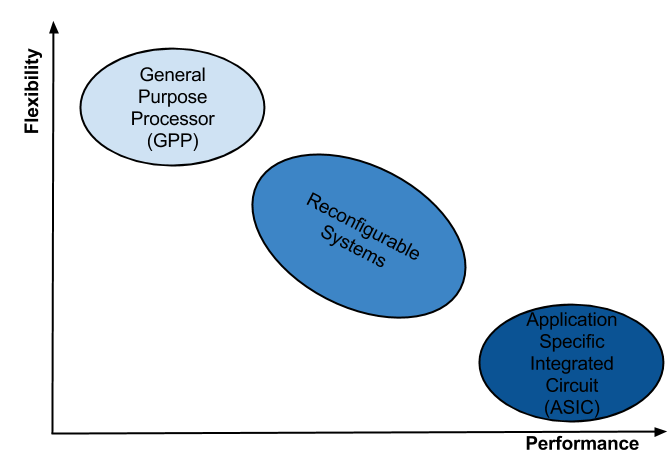
\includegraphics[scale=0.45]{Fig1}
		\caption{Flexibility Vs Performance of Hardware Classes}
		\label{fig:Fig1}
		\end{figure}

		\subsubsection{Granularity}

		Reconfigurable devices like \acs{fpga} have the configurable logic blocks(CLB) which can be configured to map the required functionality. The complexity of the function is not a concern but the number of inputs and output of the function has to be considered based on the FPGA architecture. This level of granularity in implementing the functions is called as Fine grained Reconfigurable architecture as it provides the reconfigurable granularity till lowest possible level. These reconfigurable devices are not energy efficient and the execution speed is too less than the ASIC counterpart. Another type of reconfigurable devices are the coarse grained reconfigurable architectures. These devices have the granularity at function levels. They will configure the Function blocks to achieve the efficient algorithm implementation.The Function blocks can vary from constant blocks to complex functions which are commonly used based on the application domain.   


		\subsubsection{Reconfiguration Models}
		The reconfigurable architectures need configuration of hardware.This can be at compile time or at runtime of an application as in  Fig.~\ref{fig:Fig2}.

		\begin{figure}[!htb]
		\centering
		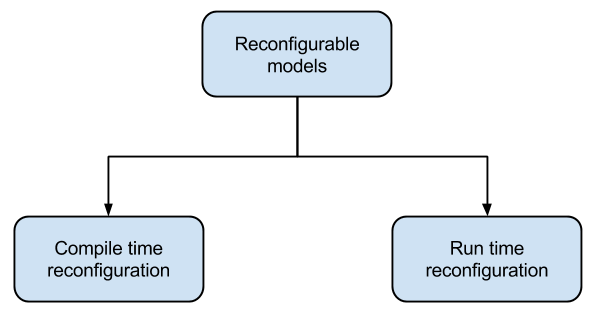
\includegraphics[scale=0.45]{Fig2}
		\caption{Reconfiguration Models}
		\label{fig:Fig2}
		\end{figure}

		In Compile time reconfiguration model, the reconfigurable hardware system is configured at compile time and will be static during the application run time.In this model the programmable logic can be configured to perform some specific task like hardware accelerators to achieve high performance.FPGA configured to perform floating point multiplication together with a GPP will accelerate the performance of the application if the GPP doesn't have a Floating Point Unit.
		In Run time reconfiguration model, the reconfiguration hardware is configured at run time and will be dynamically programmed to perform different tasks.The decision for making such dynamic reconfiguration has to be embedded coupled with the application and hence it increase the overhead.The Dynamic Reprogrammable Resource Array(DRRA) fabric developed at KTH Electronic System Dept is an example of this model\cite{5351593}.   

		\subsubsection{Reconfiguration rate}
		The Fine grain Systems will have more reconfiguration data(In FPGAs it is in term of bit streams) which leads to more time and the Coarse Grained Reconfigurable systems will have comparatively less blocks as they have higher granularity and will contain less reconfiguration data.Hence the Coarse Grain architecture will take less time to re configure. This depends on the dynamic reconfiguration architecture whether the complete fabric is reconfigured or partially reconfigured during runtime. 


		\subsection{Protocols}

		The communication between chips in Radio Base station equipments has many protocols to fulfill the requirements of the specification.The protocols differ by standards.The protocols in Data link layer of the OSI model share some common functionalities.The different protocols being used at Ericsson AB and related to this thesis work are described below:  

		\subsubsection{Ethernet}
		Ethernet is a widely used protocol for data communication.It is typically used in Local Area Network(LAN) applications.IEEE organization has standardized the protocol and revise it according to the technological advancement. The recent standard available is from 2012.The standard defines the protocol for different applications and we will consider the communication between chips in this context.  


		\subsubsection{Xio}
		Xio-s is Ericsson proprietary protocol used for communication between chips
		\subsubsection{CPRI}
		CPRI(Common Public Radio Interface) is an industry cooperation aimed at defining a publicly available specification for the key internal interface of radio base stations between Radio Equipment Control(REC) and the Radio Equipment(RE).It is the co operating work of Ericsson AB,Huawei Technologies Co.Ltd,NEC corporation,Nortel Networks SA and Siemens AG.

		\subsubsection{Protocol Functions}

		The protocols defined above are the Data link layer protocols.All these protocols have common functions which are necessary to follow the standards.The data also called payload to be transmitted need to be encapsulated or altered based on the protocol definition for successful transmission and similarly in the receiver the data will be obtained based on the protocol.Some of the common protocol functions at this level of abstraction are as below :
		\begin{itemize}
		\item{CRC Calculation and check}
		\item{Scrambling and Descrambling}
		\item{Coding and Decoding}
		\item{Framer and Deframer}
		\item{Gearbox}
		\item{Striping and Aligning}
		\item{Queues and FIFOs}
		\item{Counters}
		\end{itemize}

		\subsection{Grammar BNF}

		Bacchus-Naur form is a context free grammar used to describe the syntax of languages in computer systems.
        \\ more text to be added about the grammar

		\subsubsection{Antlr}

		ANTLR is a powerful parser generator that can be used to read,process or translate structured text or binary files.It has been adapted in academia and industries for different applications and hence there is a good community help for most common problems.The tool generates the background parser and checker files for the grammar defined in the Bacchus-Naur form(BNF)or the Extended Bacchus-Naur form(EBNF).It makes the framework easy for the user to generate a language application based on the defined grammar.

		\clearpage
		\subsection{Environment and Tools}
        The Linux based server environment is used for compiling and testing the project files.The Antlr tool is used to define the protocols in a language defined in the grammar using EBNF. The Antlr tool is made to ouput the state table information which contains all the states with transition information.This will be used to reconfigure the hardware to process the input packets according to the protocols.
        
           
        \subsubsection{SystemC}
         SystemC is an ANSI standard C++ class library for system and hardware design for use by designers and architects who need to address complex
         systems that are a hybrid between hardware and software \cite{1617814}.It helps in modeling the concurrent processes.This makes it possible to model the hardware which are concurrent systems by nature.  
        
        \subsubsection{TLM}
         Transaction level Modeling is the approach of abstracting the lower implementation details of the function units and representing the overall system architecture.TLM helps in modeling the communication and the function unit implementation separately. The Transaction refers to the set of data being exchanged.TLM speeds up the simulation by replacing a set of pin level events with a single function call.\\
         
         TLM 2.0 standard is used for the implementation of the bus system.
         
       \subsubsection{UVM}
       Universal Verification Methodology(UVM) is a verification methodology based on the best features of OVM(Open verification Methodology) and Verification Methodology Manual(VMM).A Base version of UVM is built to verify the functionality of the architecture.  
       
		\clearpage


		\section{Developed language application}
        \subsection{Hardware and interconnection}
        \subsection{Context switching}
        \subsection{Memory}
        \subsection{Error handling}
        \subsection{Transaction handling}
        
		\clearpage

		\section{Tests}
        \subsection{Complete Test System}
        \subsection{Input file}
        \subsection{Transaction routing}
        \subsection{Debugging}
        \subsection{Output}
		\clearpage

        \section{Analysis}
        \subsection{Ethernet}
        \subsection{Xio}
        \clearpage

		\section{Conclusion}
        \subsection{Limitations}
        \subsection{Future work}
		\clearpage



		\begin{filecontents*}{references.bib}


		@INPROCEEDINGS{5335678, 
			author={Szczesny, D. and Showk, A. and Hessel, S. and Bilgic, A. and Hildebrand, U. and Frascolla, V.}, 
			booktitle={System-on-Chip, 2009. SOC 2009. International Symposium on}, 
			title={Performance analysis of LTE protocol processing on an ARM based mobile platform}, 
			year={2009}, 
			month={Oct}, 
			pages={056-063}, 
			keywords={hardware-software codesign;mobile communication;mobile handsets;virtual prototyping;ARM based mobile platform;LTE protocol processing;long term evolution layer;robust header compression;Acceleration;Computational modeling;Hardware;Long Term Evolution;Mobile computing;Mobile handsets;Performance analysis;Physical layer;Protocols;Virtual prototyping}, 
			doi={10.1109/SOCC.2009.5335678},}

			@INPROCEEDINGS{558379, 
				author={Abnous, A. and Rabaey, J.}, 
				booktitle={VLSI Signal Processing, IX, 1996., [Workshop on]}, 
				title={Ultra-low-power domain-specific multimedia processors}, 
				year={1996}, 
				month={Oct}, 
				pages={461-470}, 
				keywords={computer architecture;computer networks;digital signal processing chips;integrated circuit design;land mobile radio;mobile radio;multimedia communication;portable computers;radio equipment;communication capabilities;hybrid architecture template;multimedia services;portable communication devices;portable computing;programmable devices;signal processing applications;ultra-low-power domain-specific multimedia processors;Computer aided instruction;Computer architecture;Decoding;Digital signal processing;Energy efficiency;Kernel;Multimedia computing;Portable computers;Power engineering computing;Signal processing algorithms}, 
				doi={10.1109/VLSISP.1996.558379},}

				@INPROCEEDINGS{1106752, 
					author={Keutzer, K. and Malik, S. and Newton, A.R.}, 
					booktitle={Computer Design: VLSI in Computers and Processors, 2002. Proceedings. 2002 IEEE International Conference on}, 
					title={From ASIC to ASIP: the next design discontinuity}, 
					year={2002}, 
					month={}, 
					pages={84-90}, 
					keywords={application specific integrated circuits;logic design;programmable circuits;ASIC;ASIP;Application Specific Instruction Set Processors;Application Specific Integrated Circuits;application implementation philosophy;programmable platforms;Application software;Application specific integrated circuits;Application specific processors;Computational geometry;Costs;Design methodology;Hardware;Manufacturing;Productivity;Time to market}, 
					doi={10.1109/ICCD.2002.1106752}, 
					ISSN={1063-6404},}

					@INPROCEEDINGS{6868627, 
						author={Badawi, M. and Hemani, A. and Zhonghai Lu}, 
						booktitle={Application-specific Systems, Architectures and Processors (ASAP), 2014 IEEE 25th International Conference on}, 
						title={Customizable coarse-grained energy-efficient reconfigurable packet processing architecture}, 
						year={2014}, 
						month={June}, 
						pages={30-35}, 
						keywords={application specific integrated circuits;multiprocessing systems;reconfigurable architectures;agile reconfigurability;custom ASIC implementation;customizable coarse grained energy efficient reconfigurable packet processing architecture;hardwired ASIC implementation;programmable protocol processor;real-life Voice-Over IP traffic;reconfigurable multicore packet processing architecture;retaining flexibility;time critical adaptability;Application specific integrated circuits;Delays;IP networks;Program processors;Protocols;Registers;Time factors}, 
						doi={10.1109/ASAP.2014.6868627},}

						@ARTICLE{1114865, 
							author={Estrin, G.}, 
							journal={Annals of the History of Computing, IEEE}, 
							title={Reconfigurable computer origins: the UCLA fixed-plus-variable (F+V) structure computer}, 
							year={2002}, 
							month={Oct}, 
							volume={24}, 
							number={4}, 
							pages={3-9}, 
							keywords={reconfigurable architectures;UCLA fixed-plus-variable structure computer;University of California at Los Angeles;models;reconfigurable computer architectures;reconfigurable systems analysis;reconfigurable systems design;tools;Circuits;Computer architecture;Contracts;Hardware;High performance computing;Laboratories;Mathematics;Microprocessors;System analysis and design;Telephony}, 
							doi={10.1109/MAHC.2002.1114865}, 
							ISSN={1058-6180},}

							@misc{page1985re,
								title={Re-programmable PLA},
								author={Page, D.W. and Peterson, L.V.R.},
								url={http://www.google.com/patents/US4508977},
								year={1985},
								month=apr # "~2",
								publisher={Google Patents},
								note={US Patent 4,508,977}
							}

                        @article{JACST518,
	                    author = {Abida Waza and Roohie Naaz Mir and Hakim Najeeb-ud-din},
	                    title = {Reconfigurable Architectures},
	                    journal = {Journal of Advanced Computer Science \& Technology},
                    	volume = {1},
	                    number = {4},
                    	year = {2012},
	                    keywords = {},
	                    abstract = {In the area of computer architecture, designers are faced with the trade-of between flexibility and performance. The architectural choices span a wide spectrum, with general-purpose processors and application specific integrated circuits (ASICs) at opposite ends. General-purpose processors are not optimized to specific applications; they are flexible due to their versatile instruction sets that allow the implementation of every computable task. ASICs are dedicated hardware devices that can achieve higher performance, require less silicon area, and are less power-consuming than instruction-level programmable processors. However, they lack in flexibility. Reconfigurable computer architectures promise to overcome this traditional trade-off and achieve both, the high performance of ASICs and the flexibility of general-purpose processors.},
	                    issn = {2227-4332},
	                    url = {http://www.sciencepubco.com/index.php/JACST/article/view/518},
	                    pages = {337--346}

                    	@INPROCEEDINGS{5351593, 
	                	author={Shami, M.A. and Hemani, A.}, 
	                	booktitle={ASIC, 2009. ASICON '09. IEEE 8th International Conference on}, 
		                title={Partially reconfigurable interconnection network for dynamically reprogrammable resource array}, 
		                year={2009}, 
		                month={Oct}, 
	                	pages={122-125}, 
	                	keywords={multiprocessor interconnection networks;reconfigurable architectures;binary encoding;dynamically reprogrammable resource array;innovative regular nonblocking interconnection network;low latency interconnection network;partially reconfigurable interconnection network;point-to-multipoint interconnection network;point-to-point interconnection network;sliding window connectivity;Delay;Energy efficiency;Fabrics;Multiplexing;Multiprocessor interconnection networks;Nearest neighbor searches;Parallel processing;Reconfigurable architectures;Reconfigurable logic;Signal processing algorithms;CGRA;Dynamically Reconfigurable;Interconnects;Partially Reconfigurable}, 
		                doi={10.1109/ASICON.2009.5351593},}
                    
                    
                         @comment{ Anne H�kansson, Portal of Research Methods and Methodologies for 
                             Research Projects and Degree Projects. WORLDCOMP'13 - The 2013 
                             World Congress in Computer Science, Computer Engineering, and 
                             Applied Computing, 22-25 July, 2013 Las Vegas, Nevada; USA }
                            @book{2013portal,
                                author = "Anne H�kansson",
                                title = "Portal of Research Methods and Methodologies for Research Projects and Degree Projects",
                                publisher = "WORLDCOMP'13 - The 2013 World Congress in Computer Science, Computer Engineering, and Applied Computing",
                                pages = "22--25",
                                year = 2013
                            }
                            
                           @ARTICLE{1617814, 
                               journal={IEEE Std 1666-2005}, 
                               title={IEEE Standard System C Language Reference Manual}, 
                               year={2006}, 
                               month={}, 
                               pages={0\_1-423}, 
                               doi={10.1109/IEEESTD.2006.99475},}
}


\end{filecontents*}
\bibliographystyle{ieeetr}
\bibliography{references}
\addcontentsline{toc}{section}{References}

\end{document}
